\section{Convolution}
\label{sec:convolution}

The output of a linear system is given by the convolution of its
impulse response function with the input.  Mathematically
\begin{equation}
  y(t) = \int_0^t x(\tau)r(t-\tau)d\tau
\end{equation}
This fundamental relationship lies at the heart of linear systems
analysis.  It is used to model the dynamics of calcium buffers in
neuronal synapses, where incoming action potentials are represented as
Dirac $\delta$-functions and the calcium stores are represented with a
response function with multiple exponential time constants.  It is
used in microscopy, in which the image distortions introduced by the
lenses are \textit{deconvolved} out using a measured point spread
function to provide a better picture of the true image input.  It is
essential in structural engineering to determine how materials respond
to shocks.

The impulse response function $r$ is the system response to a
pulsatile input.  For example, in Figure~\ref{fig:convolve_explain}
below, the response function is the sum of two exponentials with
different time constants and signs.  This is a typical function used
to model synaptic current following a neuronal action potential.  The
figure shows three $\delta$ inputs at different times and with
different amplitudes.  The corresponsing impulse response for each
input is shown following it, and is color coded with the impulse input
color.  If the system response is linear, by definition, the response
to a sum of inputs is the sum of the responses to the individual
inputs, and the lower panel shows the sum of the responses, or
equivalently, the convolution of the impulse response function with
the input function.

\begin{center}%
\begin{figure}
\begin{centering}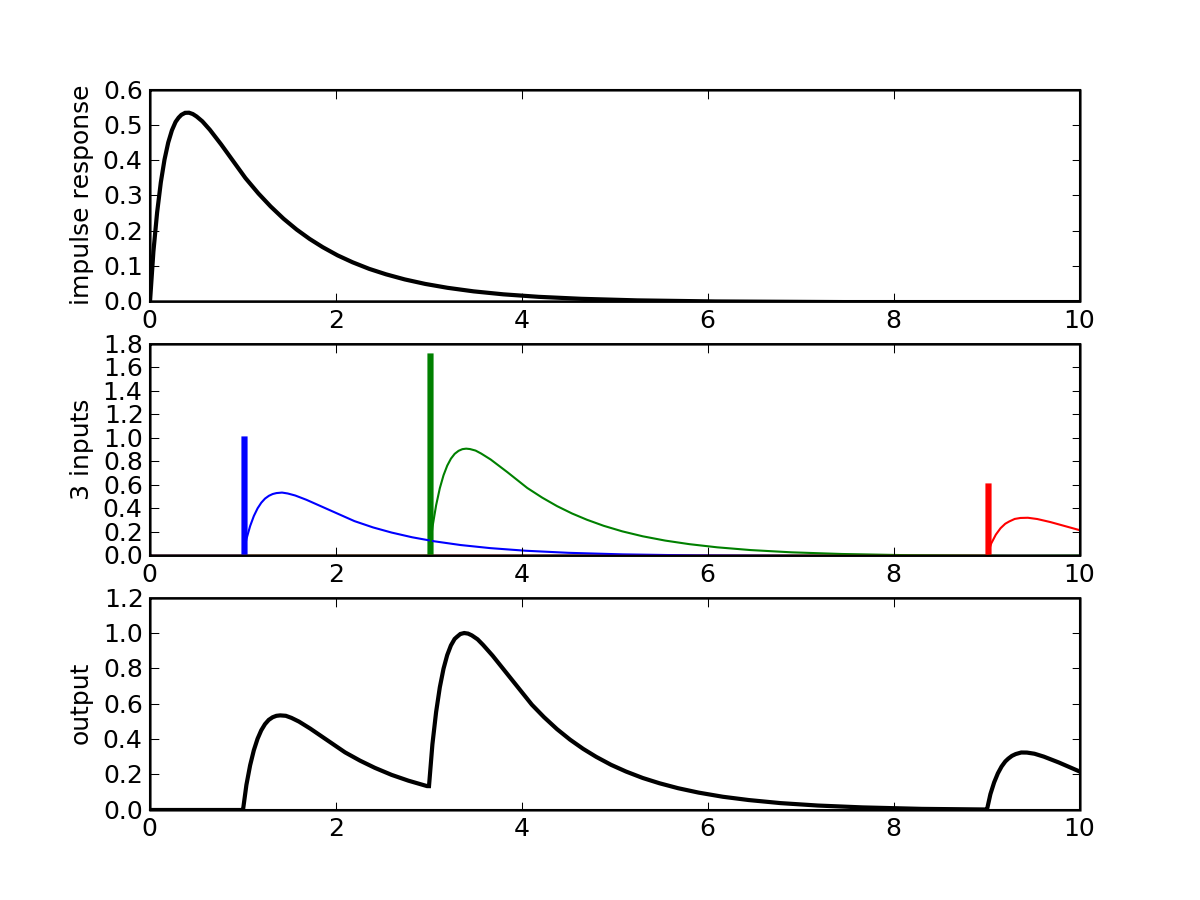
\includegraphics[width=4in]{fig/convolve_explain}\par\end{centering}
\caption{\label{fig:convolve_explain}The output of a linear system to
a series of impulse inputs is equal to the sum of the scaled and time
shifted impulse response functions.}
\end{figure}
\par\end{center}

In Figure~\ref{fig:convolve_explain}, the summing of the impulse
response function over the three inputs is conceptually and visually
easy to understand.  Some find the concept of a convolution of an
impulse response function with a continuos time function, such as a
sinusoid or a noise process, conceptually more difficult.  It
shouldn't be.  By the \textit{sampling theorem}, we can represent any
finite bandwidth continuous time signal as the sum of Dirac-$\delta$
functions where the height of the $\delta$ function at each time point
is simply the amplitude of the signal at that time point.  The only
requirement is that the sampling frequency be at least as high as the
Nyquist frequency, defined as the highest spectral frequency in the
signal divided by 2.  See Figure~\ref{fig:convolve_deltas} for a
representation of a delta function sampling of a damped, oscillatory,
exponential function.


\begin{center}%
\begin{figure}
\begin{centering}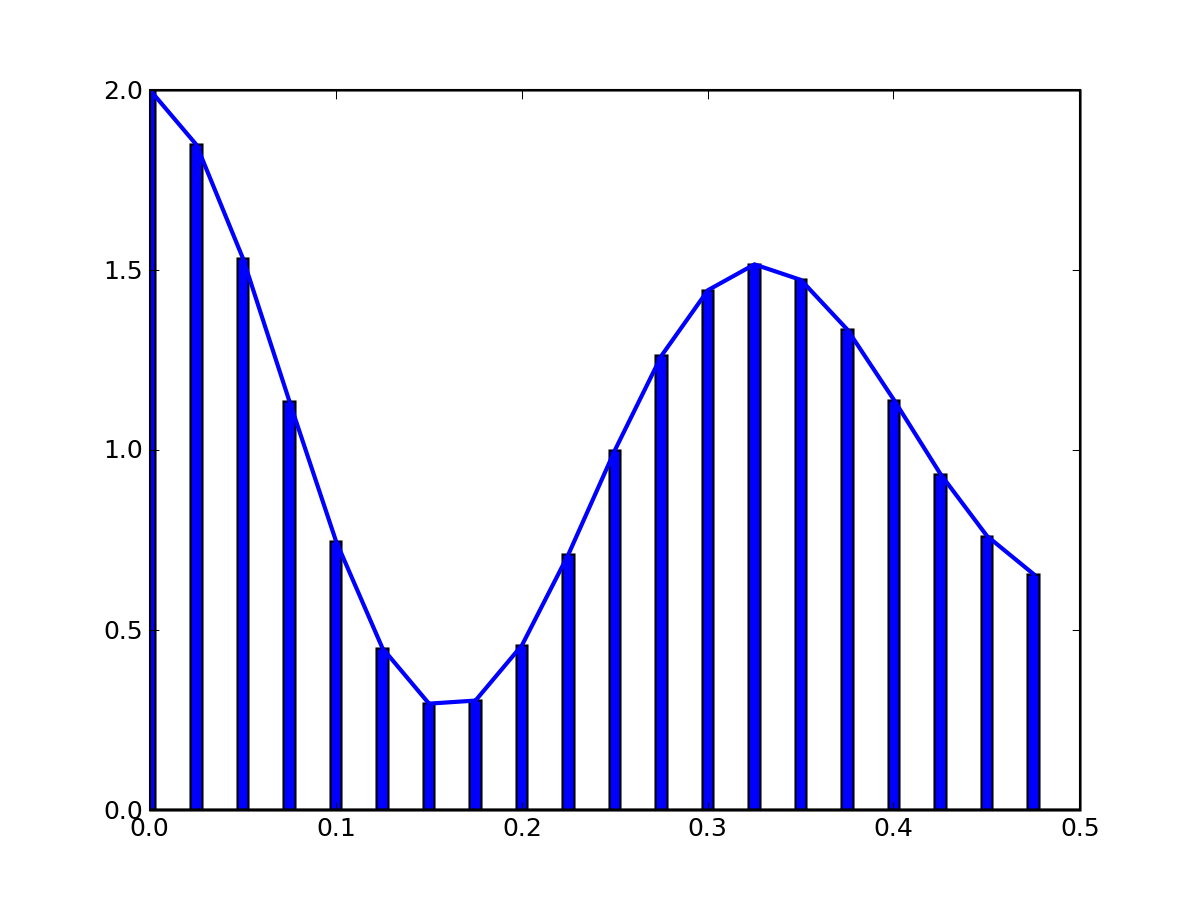
\includegraphics[width=4in]{fig/convolve_deltas}\par\end{centering}
\caption{\label{fig:convolve_deltas}Representing a continuous time signal sampled as a sum of delta functions.}
\end{figure}
\par\end{center}


In the exercise below, we will convolve a sample from the normal
distribution (white noise) with a double exponential impulse response
function.  Such a function acts as a low pass filter, so the resultant
output will look considerably smoother than the input.  You can use
\texttt{numpy.convolve} to perform the convolution numerically.

We also explore the important relationship that a convolution in the
tempoeral (or spatial) domain becomes a multiplication in the spectral
domain, which is mathematically much easier to work with.  
\[
Y = R*X
\] 

where $Y$, $X$, and $R$ are the Fourier transforms of the respective
variable in the temporal convolution equation above.  The Fourier
transform of the impulse response function serves as an amplitude
weighting and phase shifting operator for each frequency component.
Thus, we can get deeper insight into the effects of impulse response
function $r$ by studying the amplitude and phase spectrum of its
transform $R$.  In the example below, however, we simply use the
multiplication property to perform the same convolution in Fourier
space to confirm the numerical result from \texttt{numpy.convolve}.

\lstinputlisting[label=code:convolution_demo,caption={IGNORED}]{problems/convolution_demo.py}



\begin{center}%
\begin{figure}
\begin{centering}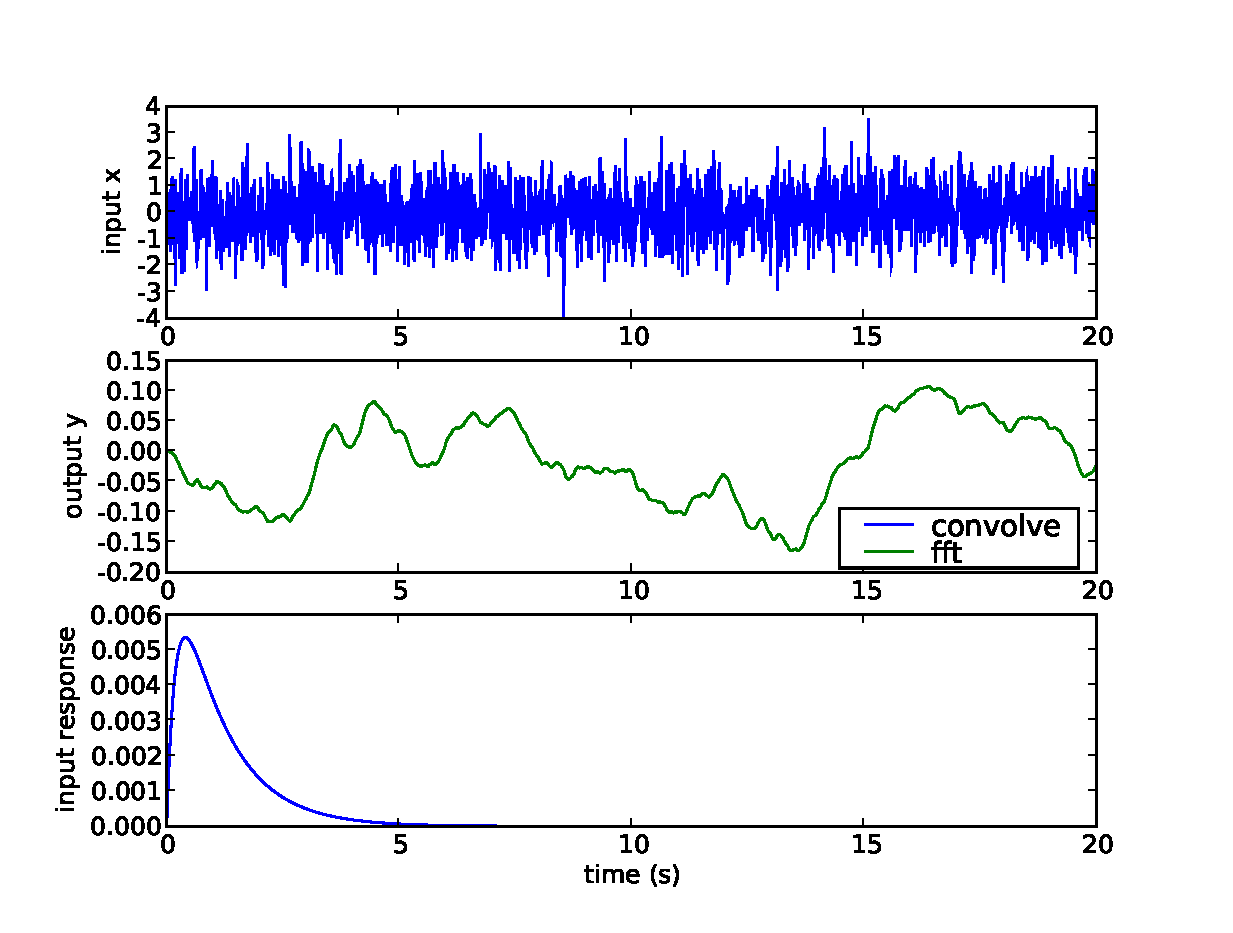
\includegraphics[width=4in]{fig/convolution_demo}\par\end{centering}
\caption{\label{fig:convolution_demo}Convolution of a white noise process with a double exponential function computed with \texttt{numpy.fft} and \texttt{numpy.convolve}}
\end{figure}
\par\end{center}
